\section{Date: 2026-07-30}
\noindent \textbf{Series ID: B1604C1A027NBEA} 

\noindent This series is titled Government social benefits: to persons: State and local: Employment and training and has a frequency of Annual. The units are Billions of Dollars and the seasonal adjustment is Not Seasonally Adjusted.The observation start date is 1974-01-01 and the observation end date is 2024-01-01.The popularity of this series is 1. \\ 

\noindent \textbf{Series ID: EEZOXSLNQ} 

\noindent This series is titled Weighted-Average Effective Loan Rate for Zero Interval, Other Risk (Acceptable), Large Domestic Banks (DISCONTINUED) and has a frequency of Quarterly, 2nd Month's 1st Full Week. The units are Percent and the seasonal adjustment is Not Seasonally Adjusted.The observation start date is 1997-04-01 and the observation end date is 2017-04-01.The popularity of this series is 1. \\ 

\subsection{Raw Regression}
\noindent Regresses the two series against each other directly. A significant result here can come just as easily from both series sharing a long-run trend as from any real relationship.

\begin{center}
\begin{tabular}{lclc}
\toprule
\textbf{Dep. Variable:}               & value\_fred\_EEZOXSLNQ & \textbf{  R-squared:         } &     0.004   \\
\textbf{Model:}                       &          OLS           & \textbf{  Adj. R-squared:    } &    -0.052   \\
\textbf{Method:}                      &     Least Squares      & \textbf{  F-statistic:       } &   0.06894   \\
\textbf{Date:}                        &    Thu, 30 Jul 2026    & \textbf{  Prob (F-statistic):} &    0.796    \\
\textbf{Time:}                        &        13:21:13        & \textbf{  Log-Likelihood:    } &   -43.377   \\
\textbf{No. Observations:}            &             20         & \textbf{  AIC:               } &     90.75   \\
\textbf{Df Residuals:}                &             18         & \textbf{  BIC:               } &     92.75   \\
\textbf{Df Model:}                    &              1         & \textbf{                     } &             \\
\textbf{Covariance Type:}             &       nonrobust        & \textbf{                     } &             \\
\bottomrule
\end{tabular}
\begin{tabular}{lcccccc}
                                      & \textbf{coef} & \textbf{std err} & \textbf{t} & \textbf{P$> |$t$|$} & \textbf{[0.025} & \textbf{0.975]}  \\
\midrule
\textbf{const}                        &       4.8395  &        3.093     &     1.565  &         0.135        &       -1.659    &       11.338     \\
\textbf{value\_fred\_B1604C1A027NBEA} &       0.6756  &        2.573     &     0.263  &         0.796        &       -4.730    &        6.081     \\
\bottomrule
\end{tabular}
\begin{tabular}{lclc}
\textbf{Omnibus:}       &  4.642 & \textbf{  Durbin-Watson:     } &    0.457  \\
\textbf{Prob(Omnibus):} &  0.098 & \textbf{  Jarque-Bera (JB):  } &    2.646  \\
\textbf{Skew:}          &  0.672 & \textbf{  Prob(JB):          } &    0.266  \\
\textbf{Kurtosis:}      &  1.830 & \textbf{  Cond. No.          } &     12.5  \\
\bottomrule
\end{tabular}
%\caption{OLS Regression Results}
\end{center}

Notes: \newline
 [1] Standard Errors assume that the covariance matrix of the errors is correctly specified.

\begin{figure}
\centering
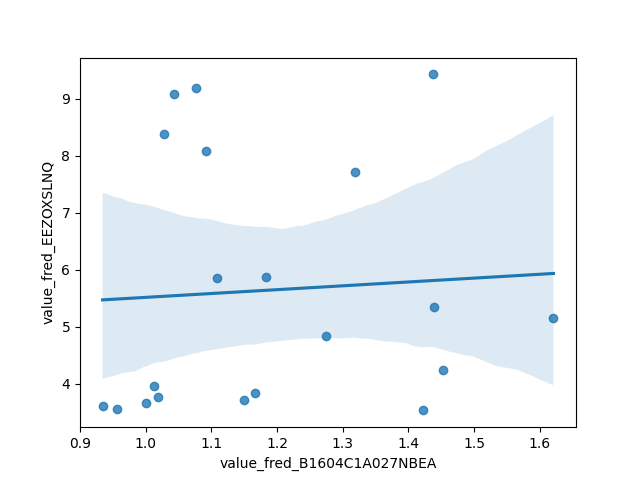
\includegraphics[scale = 0.9]{plots/plot_2026-07-30.png}
\caption{Raw Regression Plot for 2026-07-30}
\end{figure}
\newpage
\subsection{Detrended Regression}
\noindent Regresses the residuals of each series after removing its own linear time trend, so a shared trend can no longer drive the result on its own. A relationship that stays significant here is better evidence of a genuine link between the two series.

\begin{center}
\begin{tabular}{lclc}
\toprule
\textbf{Dep. Variable:}                          & value\_fred\_EEZOXSLNQ\_detrended & \textbf{  R-squared:         } &     0.217   \\
\textbf{Model:}                                  &                OLS                & \textbf{  Adj. R-squared:    } &     0.174   \\
\textbf{Method:}                                 &           Least Squares           & \textbf{  F-statistic:       } &     5.003   \\
\textbf{Date:}                                   &          Thu, 30 Jul 2026         & \textbf{  Prob (F-statistic):} &   0.0382    \\
\textbf{Time:}                                   &              13:21:13             & \textbf{  Log-Likelihood:    } &   -30.359   \\
\textbf{No. Observations:}                       &                   20              & \textbf{  AIC:               } &     64.72   \\
\textbf{Df Residuals:}                           &                   18              & \textbf{  BIC:               } &     66.71   \\
\textbf{Df Model:}                               &                    1              & \textbf{                     } &             \\
\textbf{Covariance Type:}                        &             nonrobust             & \textbf{                     } &             \\
\bottomrule
\end{tabular}
\begin{tabular}{lcccccc}
                                                 & \textbf{coef} & \textbf{std err} & \textbf{t} & \textbf{P$> |$t$|$} & \textbf{[0.025} & \textbf{0.975]}  \\
\midrule
\textbf{const}                                   &    3.395e-13  &        0.260     &   1.3e-12  &         1.000        &       -0.547    &        0.547     \\
\textbf{value\_fred\_B1604C1A027NBEA\_detrended} &      -3.2585  &        1.457     &    -2.237  &         0.038        &       -6.319    &       -0.198     \\
\bottomrule
\end{tabular}
\begin{tabular}{lclc}
\textbf{Omnibus:}       &  3.290 & \textbf{  Durbin-Watson:     } &    1.383  \\
\textbf{Prob(Omnibus):} &  0.193 & \textbf{  Jarque-Bera (JB):  } &    2.475  \\
\textbf{Skew:}          &  0.851 & \textbf{  Prob(JB):          } &    0.290  \\
\textbf{Kurtosis:}      &  2.731 & \textbf{  Cond. No.          } &     5.60  \\
\bottomrule
\end{tabular}
%\caption{OLS Regression Results}
\end{center}

Notes: \newline
 [1] Standard Errors assume that the covariance matrix of the errors is correctly specified.

\begin{figure}
\centering
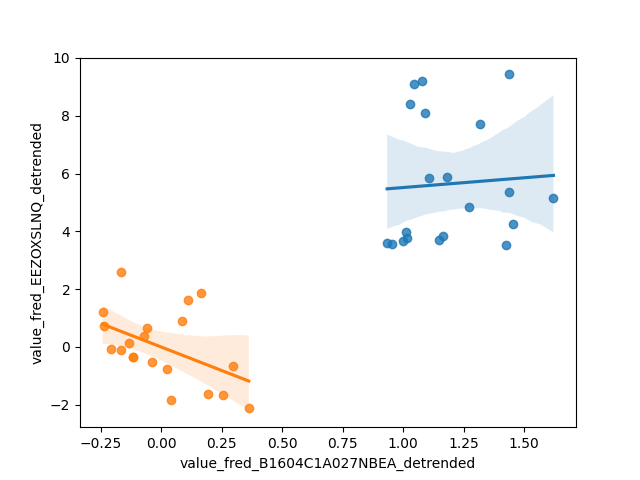
\includegraphics[scale = 0.9]{plots/plot_2026-07-30_detrended.png}
\caption{Detrended Regression Plot for 2026-07-30}
\end{figure}
\newpage
